\documentclass[sigconf]{acmart}

\usepackage[utf8]{inputenc}									% Festlegen des Encodings
\usepackage[ngerman]{babel}                                 % deutsche Sprache
\usepackage[T1]{fontenc}                                    % Unterstützung für Umlaute mit Fonts
\usepackage[autostyle=true,german=quotes]{csquotes}			% Wird für den Befehl \enquote benötigt
\usepackage{mathtools}										% Erweiterung der math-Umgebung
\usepackage{xcolor}											% Färben von Elementen wie Text

\newtheorem{Definition}{Definition}

\definecolor{my-blue}{HTML}{3D60F5}
\definecolor{my-green}{HTML}{009640}
\definecolor{my-red}{HTML}{FF2F2F}
\definecolor{my-yellow}{HTML}{ED7D31}

\begin{document}
	\title{The Serial Safety Net:\\ Efficient Concurrency Control on Modern Hardware}
	\subtitle{Seminarausarbeitung}
	
	\author{Florian Lüdiger}
	\affiliation{
		\institution{Technische Universität Dortmund}
	}
	\email{florian.luediger@tu-dortmund.de}
	\setcopyright{none}
	
	\settopmatter{printacmref=false, printccs=false, printfolios=false}
	
	\acmConference{Seminar Transaktionsverwaltung auf moderner Hardware}{Wintersemester 2017/18}{Technische Universität Dortmund}
	\acmPrice{}
	\acmISBN{}
	\acmDOI{}
	
	\maketitle
	
	\section{Einleitung}
\label{sec:einleitung}

In diesem Dokument wird das in der Veröffentlichung \enquote{The Serial Safety Net: Efficient Concurrency Control on Modern Hardware} von Wang et al. \cite{Wang:2015} vorgestellte Verfahren zur Sicherstellung der Serialisierbarkeit von Transaktionsplänen erläutert.
Dabei werden bestehende Verfahren für das Verwalten nebenläufiger Zugriffe auf eine Datenbank, allgemein als Concurrency-Control(CC) bekannt, so erweitert, dass diese die Serialisierbarkeit der entstehenden Pläne gewährleisten.
Untersuchte Verfahren sind dabei beispielsweise Snapshot-Isolation(SI), Read-Committed(RC) oder Read-Committed mit Locks(RCL).

Der Vorteil des Serial Safety Nets(SSN) gegenüber klassischen Verfahren, wie dem Zwei-Phasen-Sperrprotokoll(2PL) oder der Serializable-Snapshot-Isolation(SSI), besteht darin, dass eine bessere Nebenläufigkeit von Transaktionen ermöglicht wird, wodurch der Durchsatz des gesamten Systems massiv gesteigert wird.

\begin{figure}
	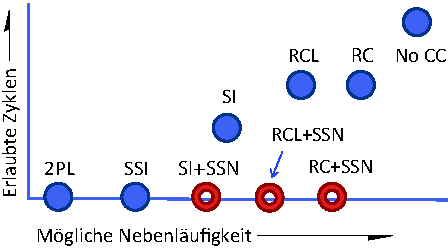
\includegraphics{img/Figure_1_komplett.pdf}
	\caption{Klassische Concurrency-Control-Verfahren im Vergleich zum Serial Safety Net}
	\label{fig:trade_off}
\end{figure}

In Abbildung \ref{fig:trade_off} wird schematisch dargestellt, dass ein bestimmter Trade-off zwischen der zugelassenen Nebenläufigkeit und den erlaubten Zyklen im Abhängigkeitsgraphen, also dem gewünschten Isolationslevel, besteht.
Klar erkennbar ist, dass ein optimales Concurrency-Control-Verfahren keinerlei Zyklen erlaubt und dennoch eine maximale Nebenläufigkeit gewährleistet.
Es wird deutlich, dass die durch das Serial Safety Net erweiterten Verfahren überhaupt keine solcher Zyklen erlauben und somit in dieser Hinsicht gleichwertig zu Verfahren wie 2PL und SSI sind.
Gleichzeitig ist allerdings erkennbar, dass die erlaubte Nebenläufigkeit wesentlich höher ist und somit ein Performanzgewinn erwartet wird.

Einige Gründe dafür, dass die bisher bekannten Verfahren zur Sicherstellung der Serialisierbarkeit, wenig performant sind, finden sich darin, dass diese einen hohen Overhead produzieren und teilweise zu unnötigen Transaktionsabbrüchen führen, wodurch möglicherweise gültige Pläne verworfen werden.
Außerdem funktionieren diese aufgrund schlechter Skalierung schlecht auf moderner Hardware, bei der immer mehr Operationen im Hauptspeicher stattfinden, wodurch die I/O-Last sinkt und damit ein noch größerer Fokus auf einem effizienten Concurrency-Control-System liegt.

Wichtig ist in diesem Zusammenhang zu erwähnen, dass ein Transaktionsplan, der in diesem Dokument als serialisierbar bezeichnet wird, keinen Schutz gegen Phantome bietet.
Das Serial Safety Net lässt sich durch das Verwenden von Sperren allerdings leicht erweitern, sodass das Vorkommen von Phantomen ausgeschlossen wird, worauf in einem die ursprüngliche Veröffentlichung ergänzenden Artikel näher eingegangen wird. \cite{WangJFP16}
Weitere Informationen zu möglichen Anomalien, Isolationsleveln und dem Phantom-Problem finden sich in \cite{Berenson:1995}.
	\section{The Serial Safety Net}
\label{sec:ssn}

Das Serial Safety Net baut auf bestehenden Multiversion-Concurrency-Control-Verfahren auf.
In einem System, welches Multiversion-Concurrency-Control(MVCC) verwendet, bestehen alle Datenbankelemente aus einer Sequenz von Versionen, wobei Schreiboperationen jeweils eine Version anlegen und Leseoperationen eine Version zurückgeben.

Für solche MVCC-Verfahren sichert das Serial Safety Net einen kreisfreien Abhängigkeitsgraphen, wodurch die Serialisierbarkeit des Transaktionsplans gewährleistet wird.
Der Abhängigkeitsgraph stellt dabei eine Übersicht über die Abhängigkeit zwischen den Transaktionen eines Plans dar, wobei die Knoten des Graphen die committeten Transaktionen und die Kanten die Abhängigkeiten zwischen diesen darstellen.
Ein Graph ohne Zyklen garantiert dabei immer, dass ein äquivalenter serieller Plan zu den ausgeführten Transaktionen existiert, welcher zum selben Ergebnis geführt hätte.

\begin{Definition}
	Die Abhängigkeit $T\leftarrow U$ zwischen den Transaktionen $T$ und $U$ besagt, dass $U$ von $T$ abhängig ist und somit $T$ als direkter Vorgänger und $U$ als direkter Nachfolger bezeichnet wird.
\end{Definition}

Es gibt zwei verschiedene Arten von Abhängigkeiten zwischen Transaktionen:
\begin{itemize}
	\item $T_i\xleftarrow{w:x}T$ - \textbf{Lese-/Schreibabhängigkeit}: $T$ greift auf eine Version zu, welche $T_i$ erstellt hat, weshalb $T$ nach $T_i$ serialisiert werden muss
	\item $T\xleftarrow{r:w}T_j$ - \textbf{Anti-Abhängigkeit}: $T$ liest eine Version, die $T_j$ überschrieben hat, weshalb $T$ vor $T_j$ serialisiert werden muss
\end{itemize}

Eine zentrale Rolle bei der Umsetzung des Serial Safety Nets spielt die Untersuchung der Abhängigkeiten von Transaktionen in Verbindung mit der Commit-Reihenfolge.
Dazu lassen sich zwei verschiedene Typen von Abhängigkeiten wie folgt definieren.

\begin{Definition}
	Bei einer \textcolor{my-green}{Back-Edge} $T\xleftarrow{b} U$ committet der Nachfolger $U$ zuerst.
\end{Definition}

\begin{Definition}
	Bei einer \textcolor{my-blue}{Forward-Edge} $T\xleftarrow{f} U$ committet der Vorgänger $T$ zuerst.
\end{Definition}

\begin{Definition}
	Eine \textcolor{my-green}{reflexive, transitive Back-Edge} $T\xleftarrow{b*} U$ bezeichnet eine Verbindung, bei der $T$ von $U$ ausschließlich über Back-Edges erreichbar ist.
\end{Definition}

\begin{figure}
	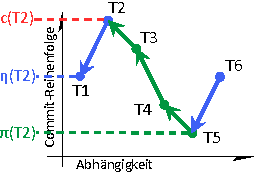
\includegraphics[width=0.8\columnwidth]{img/Figure_2_1.pdf}
	\caption{Veranschaulichung von \textcolor{my-green}{Back}- und \textcolor{my-blue}{Forward-Edges} sowie den Zeitstempeln von Transaktion $T2$}
	\label{fig:back_forward}
\end{figure}

Zum besseren Verständnis sind die genannten Begriffe in Abbildung \ref{fig:back_forward} veranschaulicht worden.
Die abgebildeten Back-Edges ergeben zusammen eine reflexive, transitive Back-Edge von Transaktion $T2$ zu $T5$.

Die Umsetzung des Serial Safety Nets erfordert das Erfassen der folgenden drei Zeitstempel zu jeder Transaktion, welche es später erlauben einen Abhängigkeitszyklus zu erkennen.
Die vorgestellten Zeitstempel sind ebenfalls in Abbildung \ref{fig:back_forward} für die Transaktion $T2$ eingezeichnet.

\begin{Definition}
	\textcolor{my-red}{$c(T)$} bezeichnet den Commit-Zeitpunkt der Transaktion $T$
\end{Definition}

\begin{Definition}
	\textcolor{my-green}{$\pi (T)$} bezeichnet den Commit-Zeitpunkt des ältesten Nachfolgers, der durch Back-Edges erreichbar ist:\\		
	$\pi (T)=\min (c(U):T\xleftarrow{b*}U)=\min (\{\pi (U):T\xleftarrow{b}U\}\cup \{c(T)\})$
\end{Definition}

\begin{Definition}
	\textcolor{my-blue}{$\eta (T)$} bezeichnet den Commit-Zeitpunkt des zuletzt committeten Vorgängers von $T$:\\
	$\eta (T) = \max (\{c(U):U\xleftarrow{f} T\}\cup \{-\infty \})$
\end{Definition}

Mithilfe dieser Zeitstempel lässt sich nun für jede Transaktion $T$ ein sogenanntes Ausschlussfenster definieren, welches garantiert, dass ein Vorgänger von $T$ nicht gleichzeitig ein Nachfolger sein kann, was auf einen Abhängigkeitskreis hinweisen würde.
Eine Verletzung dieses Ausschlussfensters durch eine Abhängigkeit $U\leftarrow T$ lässt sich feststellen, wenn ein Vorgänger $U$ gefunden wird, sodass die folgende Ungleichung erfüllt ist.

\begin{equation}
	\textcolor{my-green}{\pi (T)} \leq \textcolor{my-yellow}{c(U)} \leq \textcolor{my-red}{c(T)}
	\label{eq:ausschlussfenster_lang}
\end{equation}

Gibt es für die Transaktion $T$ also einen Vorgänger $U$, welcher nach dem ältesten Nachfolger von $T$, nämlich \textcolor{my-green}{$\pi (T)$}, committet wurde, dann kann nicht sichergestellt werden, dass $U$ nicht auch ein Nachfolger von $T$ ist.
Dies liegt daran, dass die Transaktion nichts über die Nachfolger von \textcolor{my-green}{$\pi (T)$} weiß und es somit möglich wäre, dass $U$ einer dieser Nachfolger ist, was damit einen Abhängigkeitszyklus bedeuten würde.

In dem Beispiel aus Abbildung \ref{fig:back_forward} ist erkennbar, dass für die Transaktion $T2$ eine solche Verletzung des Ausschlussfensters vorliegt, da die Transaktion $T1$, welche ein Vorgänger von $T2$ ist, zwischen \textcolor{my-red}{$c(T2)$} und \textcolor{my-green}{$\pi (T2)$} committet wurde.
Dies wird außerdem klar dadurch, dass die Transaktion $T6$ in diesem Beispiel ebenfalls die Transaktion $T1$ sein könnte, wovon $T2$ nicht direkt etwas wüsste.
Damit wäre der Abhängigkeitszyklus entstanden und der Plan nicht serialisierbar.

Um die Umsetzung des Serial Safety Nets einfacher und performanter zu gestalten, lässt sich die Ungleichung \ref{eq:ausschlussfenster_lang} noch weiter vereinfachen.
Zum einen müssen nur Vorgänger betrachtet werden, welche vor $T$ committet wurden, da ansonsten der zweite Teil der Ungleichung automatisch nicht erfüllt wäre.
Dies eröffnet die Freiheit das Überprüfen des Ausschlussfensters erst zum Commit-Zeitpunkt der betrachteten Transaktion zu durchzuführen.

Außerdem wird nur der Vorgänger von $T$ betrachtet, dessen Commit-Zeitpunkt am spätesten ist, da dieser maßgebend für das Erfüllen des ersten Teils der Ungleichung ist.
Wie vorher beschrieben wird die Commit-Zeit des zuletzt committeten Vorgängers von $T$ mit \textcolor{my-blue}{$\eta (T)$} bezeichnet, wodurch die Ungleichung \ref{eq:ausschlussfenster_lang} folgendermaßen vereinfacht wird.

\begin{equation}
	\textcolor{my-green}{\pi (T)} \leq \textcolor{my-blue}{\eta (T)}
	\label{eq:ausschlussfenster_kurz}
\end{equation}

Wird diese Bedingung auf das in Abbildung \ref{fig:back_forward} beschriebene Beispiel angewendet, wird deutlich, dass die Ungleichung für Transaktion $T2$ erfüllt ist und somit eine Verletzung des Ausschlussfensters erkannt wird.

Eine weitere hervorragende Eigenschaft des Serial Safety Nets ist die Möglichkeit des sogenannten \textbf{Safe Retry}.
Wenn eine Transaktion aufgrund einer Verletzung des Ausschlussfensters abgebrochen werden muss, so ist es durch diese Eigenschaft möglich dieselbe Transaktion direkt zu wiederholen, ohne dass derselbe Konflikt erneut auftreten kann.
Als Beispiel sei dazu angenommen, dass die Transaktion $T$ wegen einer Ausschlussfensterverletzung von Transaktion $U$ abgebrochen werden muss.
Bei erneutem Durchführen der Transaktion als $T'$ kann dieselbe Verletzung durch $U$ nicht auftreten, da der Commit-Zeitpunkt von $U$ vor dem Anfang der Transaktion $T'$ liegt und somit nach \ref{eq:ausschlussfenster_lang} keine Verletzung zu befürchten ist.

	\section{Evaluationsumgebung}
\label{sec:evaluation_umgebung}

Um die nachfolgende Evaluierung des vorgestellten Verfahrens verstehen zu können, ist ein genaueres Verständnis der Evaluationsumgebung erforderlich.
Besonders interessant sind hierbei die verglichenen Concurrency-Control-Verfahren und der verwendete Benchmark.

\subsection{Verwendete CC-Verfahren}
Für die Bewertung des Serial Safety Nets wurde dieses auf die Concurrency-Control-Verfahren Read-Committed und Snapshot-Isolation angewendet, welche beide normalerweise keine Serialisierbarkeit gewährleisten.
Verglichen wurden diese dann mit der ursprünglichen Implementierung der Snapshot-Isolation und der Optimistic-Concurrency-Control, welche beide keine Serialisierbarkeit sichern.
Außerdem wurde ein Vergleich mit der Serializable-Snapshot-Isolation durchgeführt, welche vorher dazu verwendet wurde die Serialisierbarkeit bei der Verwendung von Snapshot-Isolation zu gewährleisten.
All diese Systeme wurden von den Autoren in das Online-Transaction-Processing(OLTP)-System Silo eingebaut und auf dieser Basis verglichen.
Nachfolgend werden einige Hinweise zu den verwendeten Verfahren erläutert, welche für das Verständnis der Evaluation erforderlich sind.

\textbf{Read-Committed (RC):} Dieses Verfahren ist in Form eines Isolationslevels sehr bekannt und weit verbreitet, es finden sich daher auch viele Informationen dazu, wie beispielsweise in \cite{Berenson:1995}.
Es wird dabei immer die neueste, committete Version eines Datensatzes gelesen und daher niemals blockiert.
Bei Schreibvorgängen wird eine neue Version angelegt, die die vorhergehende Version ersetzt, was nur blockiert, falls die vorherige Version noch nicht committet wurde.
Durch dieses Verfahren werden Abhängigkeitszyklen erlaubt, allerdings werden dirty reads und lost writes \cite{Berenson:1995} dadurch verhindert.

\textbf{Snapshot-Isolation (SI):} Die Snapshot-Isolation führt alle Leseoperationen einer Transaktion auf einem Snapshot vom Beginn der Transaktion aus, wodurch deren gesamte Leseoperationen denselben konsistenten Zustand sehen.
Enthält eine Transaktion $T$ Schreiboperationen, so darf diese nur committen, wenn es keine Transaktion $U$ gibt, sodass 
\begin{itemize}
	\item $U$ zwischen Start- und Endzeitpunkt von $T$ committet, und
	\item $U$ ein Datenobjekt manipuliert hat, welches $T$ ebenfalls manipuliert hat.
\end{itemize}
Das Verfahren lässt sich nicht wie beispielsweise Read Committet in die Standard-ANSI-Isolationslevel einordnen \cite{Adya:2000}, eine vollständige Serialisierbarkeit ist allerdings nicht gewährleistet, denn es kann der sogenannte Write Skew auftreten.

\begin{figure}
	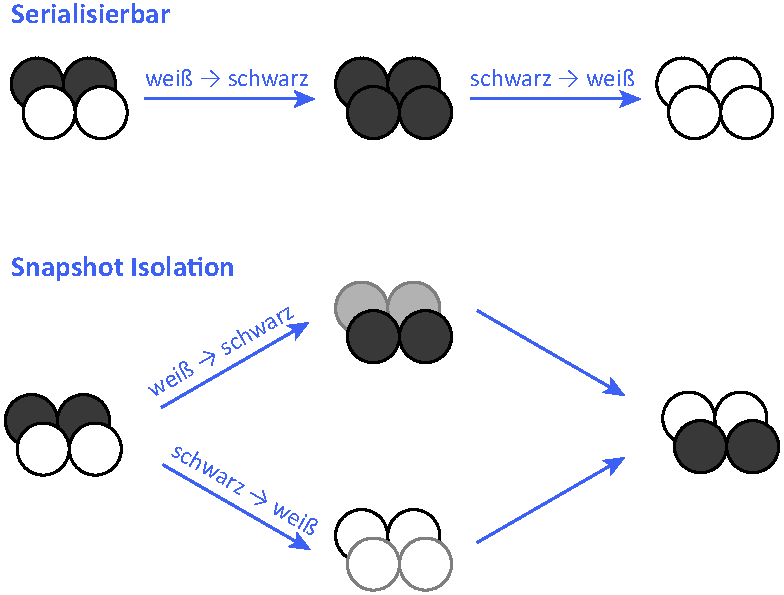
\includegraphics[width=0.8\columnwidth]{img/write_skew.pdf}
	\caption{Beispiel für das Problem des Write Skew bei der Snapshot Isolation \cite{write_skew}}
	\label{fig:write_skew}
\end{figure}

Dabei wird wie in Abbildung \ref{fig:write_skew} dargestellt über Kreuz auf Werte zugegriffen, wodurch ein anderes Ergebnis eintreten kann als bei einem entsprechenden seriellen Plan.
Im Beispiel gibt es eine Transaktion, welche alle weißen Kugeln schwarz färbt und eine andere Transaktion, welche alle schwarzen Kugeln weiß färbt.
In einem seriellen Plan würden zunächst alle weißen Kugeln schwarz gefärbt, wodurch sämtliche Kugeln schwarz gefärbt wären.
Daraufhin würden alle Kugeln von der anderen Transaktion weiß gefärbt werden, was dazu führen würde, dass sämtliche Kugeln dieselbe Farbe hätten.
Bei Verwendung der Snapshot-Isolation würden die Transaktionen gegebenenfalls parallel laufen, was dazu führen würde, dass jede Transaktion den Anfangszustand der Kugeln sehen würde, woraufhin jede Transaktion die für sie relevante Hälfte der Kugeln umfärben würde.
Nach dem Commit beider Transaktionen wäre nun immer noch die Hälfte aller Kugeln weiß und die andere Hälfte schwarz, die Kugeln hätten nur ihre Farbe getauscht, was bei einem seriellen Transaktionsplan nicht auftreten könnte.

\textbf{Serializable-Snapshot-Isolation (SSI):} Durch den geschickten Einsatz von Sperren, wird das Auftreten der vorhergehen vorgestellten Problematik bei der Snapshot-Isolation verhindert.
Somit sind bei der Verwendung dieses Verfahrens keinerlei Abhängigkeitszyklen möglich.

\textbf{Optimistic-Concurrency-Control (OCC):} Zu guter Letzt soll noch das üblicherweise in Silo verwendete CC-Verfahren untersucht werden, welches eine Variante der Optimistic-Concurrency-Control darstellt, weshalb es im Folgenden als OCC bezeichnet wird.
Dieses Verfahren sichert ebenfalls die Serialisierbarkeit des Plans und verspricht einen hohen Durchsatz sowie gute Skalierbarkeit.
Weitere Informationen zu Optimistic-Concurrency-Control und der in Silo implementierten Variante finden sich in \cite{Kung:1981} und \cite{Tu:2013}.

\subsection{Der TPC-C Benchmark}
Um die Geschwindigkeitsvorteile des Serial Safety Nets gegenüber den klassischen Verfahren quantifizieren zu können, wurde der TPC-C Benchmark verwendet.\cite{tpcc}
Es handelt sich dabei um einen Online-Transaction-Processing(OLTP)-Benchmark, welcher mehrere Transaktionstypen und eine komplexe Datenbank bietet.
Die insgesamt fünf verschiedenen Transaktionsarten modellieren dabei die Alltagsaktivitäten eines Großhandels, was das Verwalten und Ausliefern von Bestellungen, das Überwachen von Zahlungen, das Abfragen des Bestellstatus und das Beobachten des Warenbestandes umfasst.
Damit stellt dieser Benchmark eine hervorragende Simulation von stark verbreiteten Anwendungsgebieten dar, welche die Performanz des getesteten Systems in vielen Alltagssituationen einschätzen lässt.
Obwohl in dem Artikel, auf den sich diese Ausarbeitung bezieht \cite{Wang:2015} lediglich der TPC-C Benchmark betrachtet wird, ist hier anzumerken, dass die Autoren in ihrem weiterführenden Artikel \cite{WangJFP16} außerdem den TPC-CC und TPC-EH Benchmark verwendet haben um die Ergebnisse zu bestätigen.

\subsection{Testsystem}
Der Vollständigkeit halber sei hier noch erwähnt, dass zum Durchführen der Tests ein Server mit vier Sockeln verwendet wurde, der mit vier Intel Xeon E7-4807 Prozessoren bestückt war und somit über insgesamt 24 physikalische Rechenkerne verfügte.
Außerdem war das System mit 64GB Hauptspeicher ausgestattet, wodurch es sich um einen mittelgroßes Gerät handelt, wie man es beispielsweise in einem mittelständischen Unternehmen finden würde.

	\section{Evaluation}
Zur Bewertung des vorgestellten Verfahrens wird besonderes Augenmerk auf schreibintensive Transaktionen, die Performance unterschiedlicher Transaktionstypen und Commit- und Abbruchraten gelegt.
Diese Eigenschaften werden wie zuvor beschrieben mit dem TPC-C Benchmark beobachtet.

\textbf{Schreibintensive Transaktionen:} Die im TPC-C Benchmark enthaltene Payment-Transaktion stellt eine besonders schreibintensive Anwendung dar, weshalb sie für diesen Test verwendet wird.
Dabei wurde zwar der gesamte TPC-C Mix ausgeführt, allerdings wurde nur die besagte Payment-Transaktion beobachtet.

\begin{figure}
	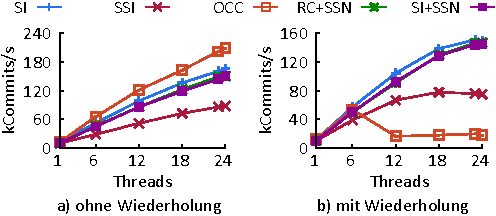
\includegraphics[width=\columnwidth]{img/Figure_3.pdf}
	\caption{Durchsatz der Payment-Transaktion des TPC-C Benchmarks}
	\label{fig:payment}
\end{figure}

Für eine differenzierte Betrachtung wurden zwei verschiedene Testszenarien beobachtet, wobei zum einen sämtliche Transaktionen, die abgebrochen werden mussten ohne eine Wiederholung fallen gelassen wurden.
Zum anderen wurde in einem Test die Performanz des Systems beobachtet wenn die fehlgeschlagenen Transaktionen direkt wiederholt werden bis diese abgeschlossen werden können.
Die Ergebnisse dieser Auswertung sind in Abbildung \ref{fig:payment} grafisch dargestellt.

Dabei fällt auf, dass die Verwendung von Read Committed in Verbindung mit dem Serial Safety Net einen Durchsatz leistet, der fast doppelt so groß ist wie der der Serializable Snapshot Isolation.
Der Grund dafür liegt laut den Autoren darin, dass der Hauptgrund für Transaktionsabbrüche bei der Verwendung von SSI in dem sogenannten Temporal Skew liegt.
Dabei versucht eine Transaktion eine Version zu überschreiben, welche nach ihrem Snapshot erstellt wurde, was bei SSI nicht zulässig ist.
RC hat damit kein Problem, da jederzeit auf die neueste Version zugegriffen wird, was sich auch durch die Erweiterung durch das SSN nicht ändert.

Außerdem ist zu erkennen, dass auch die Snapshot Isolation in Verbindung mit dem SSN eine hervorragende Performanz in beiden Testfällen besitzt.

Die Verwendung der Optimistic Concurrency Control zeigt bei dem Test ohne Wiederholungen die beste Performanz, da der gesamte Verwaltungsaufwand für die anderen CC-Verfahren entfällt.
Wird allerdings verlangt, dass die Transaktionen nach einem Abbruch wiederholt werden müssen, so sinkt der Durchsatz der OCC weit unter den Durchsatz der anderen CC-Verfahren, da die Zahl der zu wiederholenden Transaktionen so hoch ist, dass bei stark nebenläufigen Transaktionen die Performanz einbricht.
	\section{Fazit}
\label{sec:fazit}

Das Verfahren \enquote{The Serial Safety Net} verwendet hoch performante Concurrency Control Verfahren und stellt für diese die Serialisierbarkeit sicher.
Dies geschieht ohne einen besonders großen Overhead zu verursachen und führt damit zu einer hohen Performanz, wobei allerdings keinerlei Anomalien abgesehen von Phantomen entstehen können.
Die Effektivität und Skalierbarkeit in realen Systemen wurde mithilfe des TPC-C Benchmarks verifiziert, wodurch es für moderne OLTP-Anwendungen bestens geeignet sein sollte.
Außerdem ist das Verfahren unkompliziert zu implementieren, worauf in \cite{Wang:2015} genauer eingegangen wird, und somit wenig anfällig für Fehler, weshalb es als ein sicheres Verfahren gelten kann.

Das Serial Safety Net bietet insgesamt weniger Tranaktionsabbrüche, eine höhere Robustheit gegenüber dem Wiederholen von Transaktionen und ein besseres Verhalten für schreibintensive Aufgabenbereiche als die verglichenen Verfahren, wodurch einem Einsatz in realen Systemen nichts mehr im Weg steht.
	\section{Persönliche Meinung}
\label{sec:persoenliche_meinung}

	
	\bibliographystyle{ACM-Reference-Format}
	\bibliography{literatur}
\end{document}
